\chapter{State of the art}
\label{chap:sota}
\resetallacronyms

\begin{shaded}
  This chapter exposes what are the different ways to improve heat
  pump systems through a review of the available
  literature. Multistage, oil-free, and variable-speed technologies
  show promising perspectives in the heat pumps application fields and
  allow to make more efficient, more compact, more silent heat pump
  circuits built with less raw material and using a lower refrigerant
  charge.
\end{shaded}

As explained in \cref{sec:intro-slow-energy}, there are different
types of heat pumps. The interest in this chapter is focused on
electrically-driven vapor compression domestic heat pumps.

\section{Types of refrigerant compressors}

\subsection{Dynamic versus volumetric}
\label{sec:sota-dyn-vs-vol}

Refrigeration systems equipped with dynamic compressors are expected
to develop better seasonal performance than those equipped with
volumetric compressors. Indeed, soon after the scroll compressor
technology release, \citet{Purvis-1987a} described scroll-based heat
pump systems capacity response to the residential heating demand. Heat
pumps using volumetric compression devices, like scroll compressors
(the other types of volumetric compressors are even more concerned by
this trend according to \citet{ASHRAE-HVACeq-2008a-Compressor}), are
characterized by a decrease of their capacity as the outside
temperature decreases, while the residential demand evolves
inversely. This behavior explains why the heat pumps used for space or
water heating in residences must be designed to provide the heating
demand for the lowest expected outside temperature in the geographic
area. It implies that the heat pump, whose function would be to heat
the houses without any auxiliary device (like a boiler or an electric
resistor to compensate for the heat pump, or replace it totally when
outside temperature becomes too low), will be significantly
over-sized, during most of the heating period. As explained by
\citet[p.\,1922]{Schiffmann-Favrat-2009a}, variable-speed dynamic
compressors do not behave this way and stick with the residence demand
curve. They are also expected to develop better isentropic
efficiencies\footnotep{The isentropic efficiency of a compressor is
  defined in \cpref{sec:methodo-indicators}.}. Consequently using
dynamic compressors in domestic heat pump circuits would result in a
much better energy use and, potentially, in a maximization of the
efficiency, since it becomes possible to choose the exact compressor
speed which maximizes the compressor efficiency for the given mass
flow rate and pressure ratio needed. Additionally, the compression
unit would not need to be over-sized which would result in a more
rational use of raw materials and result in a smaller compression
unit, which also increases the compactness potential.

\subsection{Volumetric compressors used in domestic
  heat pumps}
\label{sec:sota-vol-cp}

The main volumetric compressor (also called positive-displacement
compressor) technologies used in refrigeration circuits are:

\begin{description}
\item[Reciprocating compressors:] Piston compressors are also known as
  reciprocating compressors. Linear stroke compressors are also
  reciprocating compressors. Historically, that compression technology
  is the first one to have powered vapor compression domestic heat
  pumps, from after somewhere between the two World Wars
  \citep[p.\,23]{zogg-2008a} to the 1980s, when the scroll compressors
  have been introduced. From that point in time, reciprocating
  compressors started to be replaced by scroll compressors in the
  domestic heat pump application. Scroll compressors were cheaper,
  more reliable, needed less maintenance, and were less noisy. In the
  1990s, most of the vapor compression domestic heat pumps are
  equipped with scroll compressors, instead of reciprocating
  compressors. Reciprocating compressors had to be lubricated to work
  properly and to not fail. With the increase of the accuracy of the
  manufacturing methods and the development of new design, linear
  stroke compressors without lubrication start to be produced. They
  target first the domestic refrigerators application, but are also
  used in some other applications, like in the study made by
  \citet{Marcinichen-Michel-2014a}. For instance,
  \citet{Marcinichen-Michel-2014a} used an oil-free 125W
  \citep[Tab.\,1, p.\,183]{Marcinichen-Michel-2014a} linear stroke
  mini-compressor capable of modulating its volumetric displacement on
  a share of the stroke \citep[p.\,183]{Marcinichen-Michel-2014a} and,
  an oil-free magnetically driven liquid gear pump to perform
  two-phase chip cooling. The compressor power of the compressor
  selected in the paper from \citet{Marcinichen-Michel-2014a} would
  not fit for domestic heating applications as its power is very
  low. Generally speaking, totally oil-free linear stroke compressors
  are limited in power range and are usually dedicated to household
  refrigerators applications, where they greatly contributed to
  increase the system performance
  \citep{Bansal-Abdelaziz-2011a}. However,
  \citet[p.\,186]{Marcinichen-Michel-2014a} consider the efficiency of
  such a compressor still low compared with conventional domestic
  heating heat pump compressors.
\item[Scroll compressors:]\label{sec:sota-scroll}A scroll compressor
  is an involute profile, mounted on a rotor, that rolls onto an other
  involute profile, which is usually fixed, and that is sightly
  offset. The involutes are drawn in a way that reduces the volume of
  the compression space further and further during the rotation of the
  shaft. The geometry of the scroll compressor has been invented by
  \citet{creux-1905a} at the beginning of the 20\th{} and did not
  really changed ever since. The involute profile is described
  mathematically by two Archimedean spirals with the same generating
  circle, and separated by a constant offset. They also can be
  generated from hybrid curves. The scroll compressor has not been
  commercialized until the early 1980s, as it had to wait for the
  development of effective high-accuracy, high volumes manufacturing
  techniques to be developed because of the complexity of the shapes
  involved \citep[p.\,16]{zogg-2008a}. Between the 1980s and 1995, the
  performance of the scroll compressors has been optimized and
  increased, then, after the introduction of the last generation of
  scroll compressors between 1992 and 1995, the increase of
  performance stopped. The data collected by
  \citet{Eschmann-2009a}\footnotep{\citet{Eschmann-2009a} performed a
    monitoring study on Brine/Water and Air/Water domestic heat pumps
    whose performance had been measured at the Swiss heat pump
    certification center between 1992 and 2007.} and summarized in his
  report of 2008 highlights the stagnation of the heat pump
  performance since the introduction of this last generation of scroll
  compressors. Nowadays development of this technology takes new
  paths, like the one explored by \citet{Iglesias-favrat-2014a}. They
  presented a prototype of oil-free scroll air compressor with two
  mobile involutes working in synchronized co-rotation one relative to
  another. The prototype can also work as a turbine, as the compressor
  is reversible. This concept could theoretically be applied with
  refrigeration compression, even if the technical challenges are
  significant. For instance, injection of liquid refrigerant during
  the compression in the volutes could also be
  done. \citet{Zehnder-2004a} has documented this kind of humid vapor
  injection in his work \citep{zehnder-favrat-2010a}, but in his case,
  one of the involutes was fixed, as he was working with an orbital
  scroll, which was making the process easier. Using co-rotative
  scrolls greatly limit the efforts on the bearings and results in a
  balanced setting \citep[Fig.\,2 p.\,567]{Iglesias-favrat-2014a},
  which makes it an interesting concept for oil-free
  applications. Nonetheless, it seems that the development of the
  scroll compressors reaches technological limits and will not
  increase its performance significantly, with the current technology
  state.
\item[Rotary vane compressors:]Rotary vane compressors are made of a
  rotor with blades inserted in radial slots in the rotor. When the
  rotor turns, the blades slide in and out of the slots, keeping
  contact with the outer wall of the compressor housing. As the rotor
  is not at the center of the housing, the gas is being compressed by
  a reduction of the volume between the blades. Those compression
  devices are being introduced recently in the domestic heat pump
  sector as a second compression stage on top of a scroll compressor
  \citep{Kondo-Kimata-2010a,Mitsubishi-2011a,Sato-Kobayashi-2012a}. A
  rotary vane compressor can be multistage and is a lot quieter than
  the reciprocating technology, at equivalent power.
\end{description}

\subsection{Dynamic compressors used in domestic
  heat pumps}
\label{sec:sota-dyn-cp}

There is no dynamic compressor technology used in the heat pump
domestic sector currently, but one is coming with the developments
performed since the beginning of the 21\th century, notably with the
work of \citet{schiffmann-2008a}.

\paragraph{Radial compressors}

The first radial compressors were manufactured at the beginning of the
$20^{\text{th}}$ century. They were originally developed by steam
turbine manufacturers and were widely used for ventilation purposes in
deep mining. At that time, the possibilities of producing an impeller
were rather limited by the manufacturing technology available. Decades
later, the manufacturing technologies had evolved and started to allow
the manufacturing of highly efficient radial compressors. Carrier has
been the first to work seriously on radial compressors from 1911 for
refrigeration applications (at the time, it was for air
conditioning). In about 1919, he first tried a German radial
compressor with di-chloroethylene, and then a compressor made by
Eastman Kodak in the United States with dichloromethane
\citep[p.\,16]{zogg-2008a}. They have been used in industrial
refrigeration circuits from the beginning of the 20\th{} century to
nowadays, and they now can be used in domestic heat pump applications
due to the recent development of the manufacturing processes and the
development of small scale gas bearings sets specially designed for
this application, with an integrated-design approach
\citep{schiffmann-2008a}.

\subsection{About the compression units used in this thesis work}
\label{sec:sota-jurg-cp}

\citet{Schiffmann-Favrat-2009a} presented in 2009 really encouraging
experimental results with the testing of a single-stage compression
unit. They also presented promising preliminary simulation results for
a twin-stage heat pump based on the radial compressor unit that
\citet{schiffmann-2008a} was developing. That compression unit, and
its successors, the twin-stage compression units used in this thesis
work, are at the cutting edge of the technique and the technology
reachable nowadays, as shown in \cref{fig:zwyssig}. Those compression
units are several times lighter and smaller than their equivalent in
the scroll technology, as illustrated in
\cref{fig:cp-unit-volume-comparison} and are expected to demonstrate
the greatest potential in many processes where gas compression is
needed. A similar design has been used by
\citet{demierre-wegele-2014a} with a compressor-turbine unit, using a
radial compressor and a radial turbine, mounted at the two sides of a
same shaft\footnotep{Details about this specific design can be found
  in the thesis work of \citet{demierre-2012a}.}. The twin-stage
compression units powering the \AWP{} and the \BWP{} have been
developed between 2002, when the feasibility study of the twin-stage
unit has been presented by \citet{schiffmann-godat-2002a}, and 2012,
when the first compression unit prototype has been able to power a
heat pump cycle in an experimental setup. The results of those first
experiments are presented in \cpref{chap:awp}.

\begin{figure}[htbp]
  \centering
  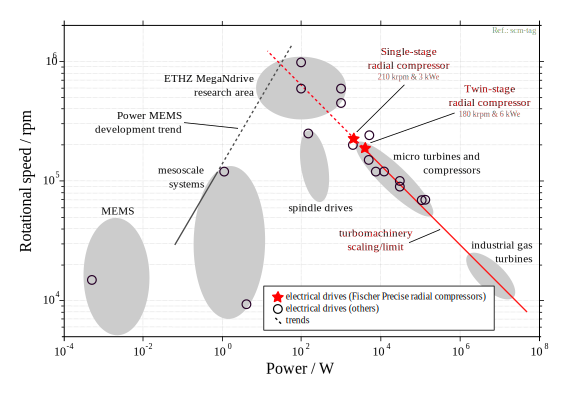
\includegraphics[width=\textwidth]{zwyssig-round-2009a-fig1p565-augmented}
  \caption[Trends for high speed electrical drives and
  turbomachineries.]
  {Emerging application areas and trends for high speed electrical
    drives and turbomachineries, based on the work of \citet[Fig.\,1,
    p.\,565]{zwyssig-round-2009a}.}
  \label{fig:zwyssig}
\end{figure}

\begin{figure}[htbp]
  \centering \subfloat[Compression unit aside a 1.5-liter water bottle]
  {\label{fig:cp-unit-1L}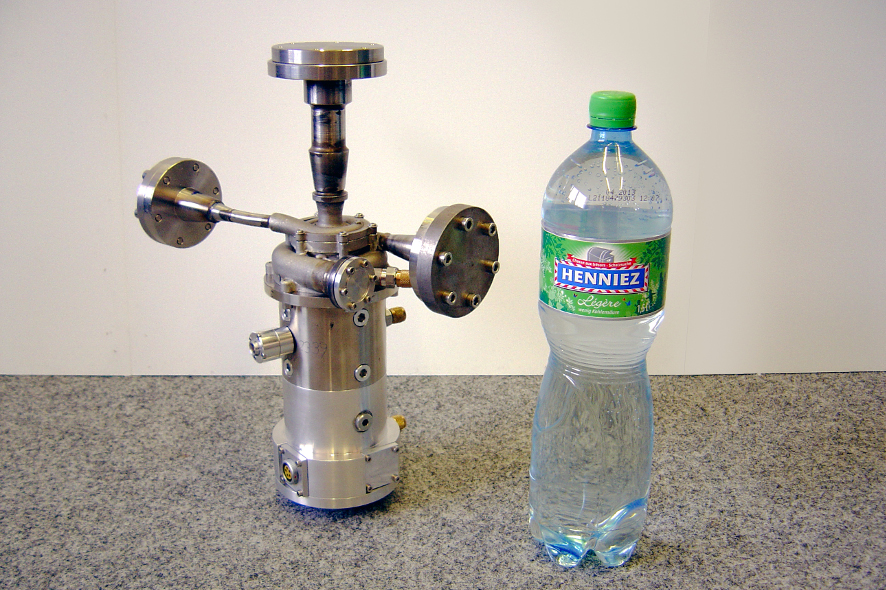
\includegraphics[width=0.45\linewidth]{20121219T094101-00066bis}}
  \hspace{1em} \subfloat[The compression unit is equivalent to 2 scroll
  compressors]
  {\label{fig:cp-unit-scrolls}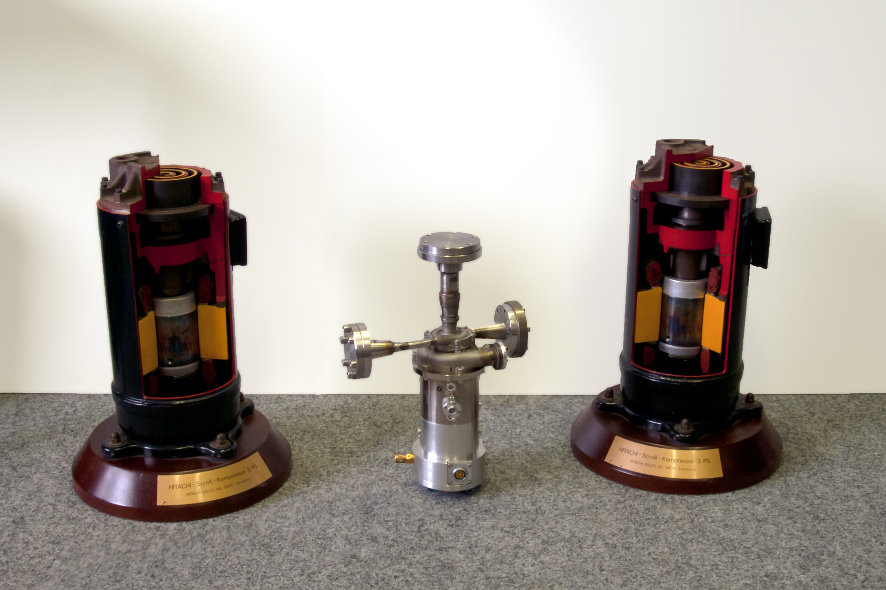
\includegraphics[width=0.45\linewidth]{20121218T525614-0049+0050}}
  \caption[Volume of the twin-stage compression unit]{The volume and
    the weight of the twin-stage compression unit are several times
    lower than a single-stage scroll compressor. The 6 kW twin-stage
    compression unit is roughly equivalent to 2 single-stage 3 kW
    scroll compressors.}
  \label{fig:cp-unit-volume-comparison}
\end{figure}

\section{Noise reduction in refrigeration circuits}

As very accurately balanced and high rotation speed devices, the
compression unit developed by \citet{schiffmann-2008a} and its
successors produce no vibrations and can be made very silent. In
opposition to typical scroll compressors that produce a lot of
vibrations and noise (about 65 dBA, on average, according to
\citet{ARI-270-94} compliant measurements, at the nominal compressor
speed of 50 Hz \citep[Fig.\,43,
p.\,37.26]{ASHRAE-HVACeq-2008a-Compressor}), widely spread on the
audible sound spectrum. This implies that this noise is difficult to
insulate, on the contrary to the radial compression units, which
produce high frequency noises due to their high rotational speed and
the gas bearings technology (no friction). As those high frequencies
are easy to staunch with basic sound insulation, radial compression
unit rotating on gas bearings can be made very silent. Furthermore,
regular Air/Water domestic heat pumps available in th
\citet{Eurovent-2010a} database release between 53 and 83 dBA (with
fans), according to ISO\,9614 \citep{EN-ISO-9614-1} ans ISO\,3744
\citep{ISO-3744-2010a} compliant measurements. Consequently,
compressor noise constitutes a significant part of the heat pump
noise. Thus, switching to radial compression unit rotating on gas
bearings and to silent fans open the way to very quiet heating
machinery.

\section{Variable-speed in refrigeration circuits}

Variable-speed capacity control has been proven to increase heat pump
efficiency \citep{Karlsson-2003a,Karlsson-Fahlen-2008a}. There are
different ways to obtain this capacity control.

Heat pump capacity control is performed by reducing the compressor
capacity.  In domestic heat pumps, most of the compressor used are
scroll compressors.  Those device are currently using one of the three
technologies detailed below to control their capacity.

\paragraph{Variable displacement based capacity control:}

This mechanism is dedicated to scroll compressors and consists in
ports incorporated in the fixed scroll. The control consists in the
connection or not of the compression chamber to the suction side by
respectively closing or opening the ports. Then, when the
ports are all closed, the compressor runs at its full
capacity. To provide only a share of the full capacity, some holes are
open. The number of different capacities and extent of the capacity
reduction available is governed by the locations of the ports.

\paragraph{Pulse Width Modulation based capacity control:}

This mechanism is also dedicated only to scroll compressors and
consists in a device that modulates the axial pressure that maintains
sealing contact between the scroll tips and its base. The control is
done by cycling the loading and unloading of the fixed scroll without
changing the motor speed.  The cycle is controlled by an electrical
devices which adapt the loading and unloading phases to make the
compressor deliver the exact capacity required.

\paragraph{Variable speed based capacity control:}

The compressor is driven by an inverter to convert the 50 Hz
fixed-frequency alternative current coming from the power network to
an adjustable voltage and frequency signal. This signal is then used
to control the speed of the motor, which is correlated with the mass
flow rate of the refrigerant through an equation or a compression
map. This capacity control strategy is used on some scroll compressors
and is the solution selected for the control of the radial compression
units used in this thesis work.

\section{Multistage refrigeration circuits}
\label{sec:sota-multistage}

Two-stage compression cycles has been proved to reach higher
performance than single-stage cycles in various studies
\citep{Favrat-Courtin-1997a,Zehnder-2004a}. Moreover, this statement
is particularly true for high temperature differences between the hot
source and the cold source. \citet{Zehnder-2004a} presented several
twin-stage heat-pump configurations and tested some of them
\citep{Zehnder-Favrat-1998a,Zehnder-Perevozchikow-2002a}. The most promising cycles were the
following:

\begin{description}
\item[Solution \#1:] Addition of a separate single-stage heat-pump
  cycle to a main single-stage heat-pump cycle. The main cycle is
  dedicated to the heating of the house while the additional cycle
  uses the subcooled liquid at the outlet of the main condenser as a
  cold source to produce tap water.
\item[Solution \#2:] Superposition of two single-stage heat-pump cycles
  coupled with a shared heat exchanger acting as the condenser for the
  bottoming cycle and an evaporator for the topping cycle.
\item[Solution \#3:] A single-stage cycle using a single-stage
  compressor with intermediate vapor-injection.
  \begin{description}
  \item[\#3.1:] The vapor injected during the compression process is
    produced by the expansion of subcooled liquid removed at the
    outlet of the condenser. Before being injected, the wet vapor is
    heated up by going though an intermediate heat exchanger,
    exchanging heat between the main subcooled liquid line and the wet
    vapor previously expanded
    \citep{Zehnder-Favrat-2002a,Beeton-Pham-2003a}. When the vapor
    exchanges heat in the intermediate heat exchanger, its vapor
    quality increases. Often, the vapor injected in the compressor is
    just saturated. Wet vapor injection is only needed if the outlet
    temperatures are getting too high.
  \item[\#3.2:] The subcooled liquid coming from the condenser is
    expanded to an intermediate pressure and enters a flash tank where
    vapor and liquid are separated. Liquid is expanded and enters the
    evaporator while vapor is injected in the compressor, during the
    compression process.
  \end{description}
\item[Solution \#4:] A twin-stage heat-pump using a twin-stage
  compressor and an intermediate heat exchanger or a flash tank in
  order to inject vapor between the two compression stages, as in the
  two versions of the above solution.
\end{description}

\citet{Schiffmann-Favrat-2005a} have analyzed those different concepts
in order to design a domestic, high temperature lift, air-water heat
pump. They sum up those concepts in a later article
\citep{Schiffmann-Favrat-2009a} and conclude notably that the solution
\#4, with a flash tank acting as an economizer, is the most
interesting one, when taking in account the radial compressors
characteristics and limitations. Moreover, they pointed out that this
solution is an elegant one in terms of number of components and
control, and a promising one in term of \COP{}
\citep{schiffmann-2008a,Favrat-Courtin-1997a}. They also indicate
that, with this cycle configuration, inverting the cycle in order to
defrost the evaporator, could allow to use the economizer as an
internal energy source. Since the final goal is the development of a
twin-stage oil-free air-water heat-pump using a twin-stage radial
compressor rotating on gas bearings, the configuration \#4 is
favored. This configuration is referred as a twin-stage compression
cycle with flash cooling, as it has been named by the ASHRAE
\citep[Fig.\,49, p.\,37.29]{ASHRAE-HVACeq-2008a-Compressor}.

\section{Lubrication in refrigeration circuits}

\citet{YoubiIdrissi-Bonjour-2008a} highlight that, currently, almost
every refrigeration vapor compression systems need a lubrication
agent, which is generally a mineral or synthetic lubricant oil
depending on the refrigerant used in the system. Oil functions are (1)
to protect the mechanical moving elements against the wear with a thin
lubricant film, (2) to act as a sealing element, (3) to limit the
noise made by the mechanisms, (4) to help the evacuation of chemical
impurities or deposits which may be present in the circuits, and (5)
to act as a heat transfer medium for cooling the compressor, in many
systems. Those favorable or vital functions clearly assert that oil in
refrigeration compression systems is generally compulsory and
useful. However, that oil brings also severe drawbacks to the
refrigeration circuits. Most of the time, it reduces the heat transfer
coefficient in heat exchangers, it changes the flow configurations, it
increases the pressure drops, and it modifies the thermodynamic
equilibrium and the thermodynamic properties of the refrigerant
\citep{YoubiIdrissi-Bonjour-2008a}.

\subsubsection{Migration of the oil inside the heat pump loops}
\label{sec:migration}

\citet{Zehnder-2004a} studied the migration of the oil into a
twin-stage heat pump loop. He concluded that the oil is migrating from
the topping stage compressor to the bottoming stage compressor and
could not identify a stable situation where this statement was
false. The topping compressor, a scroll compressor, without lubricant
oil recovery circuit, dries and is doomed to failure. Moreover,
\citet{Navarro-Corberan-2005a} studied the oil circulation ratio and
its return to the compressor with R290/\POE{} and R407C/\POE{}, on a
reciprocating compressor installation and compared their results with
mineral oil experiments. They found that the oil would return easier
to the compressor if it is a \POE{} than if it is a mineral oil. They
concluded also that there is no behavior difference, from the oil
point of view, with R290 or R407C but this conclusion is deduced from
a single-stage heat pump loop. \citet{Winandy-Cuevas-2003a} has
studied the oil level in two scroll compressor in parallel, in a
refrigeration installation. They demonstrated that the oil was not
returning equally to the two compressors, especially when working
under part load. They also linked the two compressor housings with a
straight pipe, welded at the normal height of the oil-levels, allowing
an oil-level adjustment between the two compressors and concluded the
oil migration phenomenon has to be taken seriously, even more
seriously when running under part-load. Unfortunately, in twin-stage
heat pumps based on 2 scroll compressors, since the pressure level is
not the same for the two compression devices, in opposition to the two
scroll compressors in parallel presented by
\citet{Winandy-Cuevas-2003a}, this solution is not applicable. The
direct consequence of those studies is that it should be a lot easier
to make multistage heat pump devices without having to consider the
return of the lubricant agent to the compressors. Those heat pumps are
likely to be more reliable also, as they won't fail because of
lubrication issues. Additionally, using oil-free circuits allows to
get free from the design rules of circuits with oil. For instance, the
pipe diameters can be increased in the suction lines in order to
decrease the pressure drop on the vapor line, generating exergy
losses\footnotep{Exergy and exergy efficiency are defined in
  \cpref{sec:methodo-indicators}.}. Those pipes diameters are limited
in the circuits with oil because the oil has to be recovered in the
compressor housing \citep{kesim-ileri-2000a,Guo-Shen-2011a}. This
problem is even more acute with variable flow capacities linked to
variable speed compressors.

\subsection{Impact of the lubricant on the expansion process}
\label{sec:oil-dv}

\subsubsection{Electronic expansion valves}

\citet{Liang-Zhijiu-2009a} have established models of electronic
expansion valves for R22, R407C and R410a based on Bernoulli equation
giving accurate results. The models they propose differ from some
conventional models using the two-phase outlet pressure and corrected
flow coefficient since they consider metastable phenomenona caused by
rapid depressurization and employ the throat pressure of the
electronic expansion valves and the single-phase incompressible flow
coefficient. \citet{Park-Kim-2007a} have used a different approach
using a model with a set of parameters and variables including the
valve geometry, its inlet and outlet conditions, and the refrigerant
thermodynamics properties to describe the valves behavior. Both of
those studies are dealing with pure refrigerant or neglect the
presence of oil. For now, influence of oil seems not to be documented
or considered as negligible, but it could be a problem with oil-free
circuits.

\subsubsection{Capillary tubes}

There are two groups of studies dealing with the effect of oil in the
capillary tubes. The first deals with oil-rich mixtures, with
typically more than 5\% in weight, while the second treats the oil as
a contaminant, present in quantities lower than 5\% in weight. The
studies where important quantities of oil are mixed with the
refrigerant are quite seldom but are interesting to understand and
interpret the foaming phenomenon occurring in compressors, as the oil
concentration is the highest in those devices. For instance,
\citet{Poiate-Gasche-2006a} studied the foaming phenomenon inside
small tubes. The second case is more usual and several studies have
been published. Most of them aim to improve the knowledge available on
the phenomena which occur in capillary tubes, like two-phase flow
pressure drop or metastable flow\footnotep{A metastable flow remains
  liquid over a distance longer than the one predicted by conventional
  pressure drop models.}. \citet{Motta-Braga-2002a} performed visual
experiments to determine the position of the vaporisation point of a
R404a-oil mixture inside a capillary tube and quantified the effect of
a given percentage of oil on the capillary tube behavior. Some of the
studies observed a reduction in the mass flow rate with an increase of
the oil concentration \citep{Motta-Parise-2001a,Fukuta-Ogi-2003a}.

\subsection{Impact of the lubricant on the evaporation
  process}
\label{sec:oil-ev}

The evaporation process is known for decades to be the more sensitive
process of the heat pump cycle regarding the presence of compressor
lubrication oil in the refrigerant. \citet{McMullan-Murphy-1992a} have
shown that the viscosity of the lubrication oil has a negative effect
on the evaporator performance for a fully miscible oil-refrigerant
mixture. For shell-and-tubes evaporators, they concluded that the
addition of oil produces a change in the refrigerant two-phase flow
regimes and a decrease of the overall evaporator performance. Previous
studies
\citep{McMullan-Hughes-1988b,McMullan-Hughes-1988a,Hughes-Morgan-1984a,Hughes-Morgan-1982a,Hughes-Sutcliffe-1980a,Hughes-Morgan-1984b},
observed the lubricant oil influence on the heat pump performance and
concluded that the presence of oil in the evaporator was responsible
of a significant decrease of performance. They also concluded that the
accumulation of oil at the end of the evaporator (refrigerant
vaporizes, oil just flows), has a significant influence on the
decrease of the heat transfer coefficient which is observed. They have
estimated that, in principle, an evaporator working with no oil at all
would allow an increase of the whole evaporator heat exchange
coefficient by about 40\%
\citep[p.\,123]{McMullan-Morgan-1983a}. Indeed, the more refrigerant
evaporates, the more the remaining liquid refrigerant is charged in
oil, and the more it is difficult for it to evaporate. The potential
improvement of 40\% is certainly quite optimistic, but it remains that
improvements of the heat exchange coefficient are observed with the
decrease of the oil mass faction. If oil can not be removed, from an
heat exchange point of view, \citet{McMullan-Morgan-1983a} added that,
for low amounts of oil in the refrigerant, a low viscosity oil leads
to better results, while for bigger amount of oil in the refrigerant,
high viscosity oil would be the better choice. They also observed that
the presence of oil increases the pressure drop into the
evaporator. \citet{Spindler-Hahne-2009a} have studied the influence of
oil on nucleate pool boiling heat transfer with enhanced surface
tubes. They concluded that, except under very specific conditions, oil
always decreases the heat transfer coefficient \citep[Fig.\,19
p.\,990]{Spindler-Hahne-2009a} and \citep{Moller-1998a}. The more oil
there is, the less efficient the evaporation is.
\citet{Nidegger-Thome-1997a} and \citet{Zurcher-Favrat-1998a} have
studied the intube flow boiling of R-407C and R-407C-oil mixtures
\citep{Zurcher-Favrat-1998a,Zurcher-Favrat-1998b}, and the R134a and
R134a-oil mixtures \citep{Zurcher-Favrat-1997a,Nidegger-Thome-1997a},
both on plain tubes and microfins tubes, and confirmed the
observations of \citet{McMullan-Morgan-1983a}: with increasing oil
concentration, the heat transfer coefficient drops. Some authors, like
\citet{Cawte-Poland-1996a}, observed, in the contrary, an increase of
the heat transfer if the oil concentration reaches a certain range (2
to 10\% in the case of the study published by
\citet{Cawte-Poland-1996a}). \citet{BandarraFilho-Thome-2009a}
reviewed a great number of papers involving refrigerant–oil mixtures
that can be found for different test conditions and found that they
often present conflicting results, unfortunately. Even so, it is still
possible to affirm that some thermodynamic properties of
refrigerant/oil mixtures, such as density, viscosity, surface tension
and miscibility, can modify, specifically, the heat transfer and
pressure drop, and thus affect directly the \COP{} of the system
\citep[p.\,186]{BandarraFilho-Thome-2009a}. \citet{Cawte-1992a}
performed similar heat transfer studies on condensation processes with
refrigerant/oil mixtures and observed a big non-linear decrease of the
heat coefficient with the increase of the oil concentration. However,
he concludes that this change of heat transfer coefficient has little
impact on the whole heat pump performance. Of course, it is important
to consider that most of those studies have been made on plain tubes,
or conventional surfaces.

\subsection{Oil-free heat exchange technologies}
\label{sec:sota-oilfree-hx}

Using oil-free compression devices opens the way to the use of
existing or to-develop heat exchangers, which would be more efficient
or become usable with oil-free compression technologies. Those heat
exchangers include micro-channels heat exchangers, direct ground
evaporators, and heat exchangers using enhanced surfaces, like
enhanced tubes-based heat exchangers
\citep{Ribatski-Jacobi-2005a,Habert-2009a,vanrooyen-2011a} or enhanced
plate-based heat exchangers \citep{Furberg-2006a}, which would result
in a reduction of the heat exchange surfaces, and consequently, in a
reduction of the pressure drops inside the circuits and of the whole
heat pump size. Furthermore, some of those heat exchange technologies
open the way to heat exchangers with reduced temperature pinches
between the refrigerant and the heat source and would contribute to
decrease the exergy losses coming from the heat
exchanges. \citet{Furberg-2006a} and \citet{Li-2008a} develop plates
heat exchangers with enhanced surfaces with micro patterns
\citep{Furberg-Muhammed-2009a}. Enhanced surfaces with micro-patterns
are filled with oil, if used with refrigerant-oil mixtures
\citep[Fig.\,10\,\&\,11 p.\,985--986]{Spindler-Hahne-2009a} and
thereby become less efficient. Consequently, the enhanced plate heat
exchangers developed by \citet{Furberg-Muhammed-2009a} mainly target
oil-free applications. Oil free heat exchange technologies are in
heavy development since the last 20 years \citep[Fig.\,1
p.\,186]{BandarraFilho-Thome-2009a}, as new market applications
emerge. Their application in oil-free compact domestic heat pumps
promises to increase even further the potential of the oil-free
compression technologies.

\subsection{Impact of the lubricant oil on the
  compression process}
\label{sec:oil-cp}

One of the main effect of oil in the compression process is the
foaming phenomenon, which is due to the interactions between the oil
and the refrigerant induced by the blade rotation or the vapor
blow. The foaming phenomenon has been studied in a hermetic casing
simulating a hermetic rotary compressor by
\citet{Yanagisawa-Fukuta-1991a}. They observed that the foaming
increases and become massive for high compressor blade speed combined
with a high mass flow rate. Another effect of the oil on the
compression process is the modification of the compressor
performance. Indeed, because of the solubility of the oil into the
refrigerants\footnotep{The solubility of the oil into the refrigerant
  is proved to increase with pressure
  \citep{Wahlstrom-Vamling-1997a}.}, the refrigerant-oil mixture
enthalpy may be substancially different from the pure refrigerant
enthalpy \citep[Fig.\,2--4,
p.\,288--289]{YoubiIdrissi-Meunier-2003a}. As a consequence, the
energy balance performed on the compressor may be false and, as shown
with the \citet[Fig.\,2--4, p.\,288--289]{YoubiIdrissi-Meunier-2003a}
diagrams, it leads to wrong estimations of the refrigerant mass flow
rate. Indeed, considering pure refrigerant instead of the real
oil-mixture that really flows out of the compressors leads to make a
mistake on the enthalpies at the inlet and the outlet of the
compressors, which is reflected on the energy balance, and finally on
the mass flow rates. As some refrigerant remains dissolved in the oil,
some liquid desorbs from the oil during the compression process,
inducing a wet compression process. This phenomenon may considerably
affect the compressor isentropic efficiency while it has no effect on
the volumetric efficiency \citep{Wang-Dickson-2006a}.


\section{Refrigerant charge reduction in
  refrigeration circuits}

Because of their impact on the environment, European regulation
concerning refrigerating systems has become more and more severe and
imposes increased constraints related to the refrigerant charge of the
installations. As a consequence, many studies aimed at minimizing the
charge in refrigeration circuits were developed. Studying the behavior
of the refrigerant charge in the refrigeration circuits and components
aims at understanding it and reducing the charge to its minimal
amount. \citet{Poggi-Bontemps-2008a} made a review of the studies
aiming at reducing the refrigerant charge. They conclude that the
optimal charge for each installation can be determined and that a
reduction of the overall charge can be achieved by reducing the
internal volume of exchangers, receivers, and liquid lines. In
particular, exchangers with small internal volume should be used;
compact exchangers (for instance based on the small channel
technology) allow a considerable benefit without performance decline
\citep[p.\,367]{Poggi-Bontemps-2008a}. \citet{Poggi-Bontemps-2008a}
explain also that the use of electronic expansion valves allow to
decrease the charge. The use of secondary circuits, when possible,
also helps. \citet{Palm-2007a} arrived previously to the same
conclusions than \citet{Poggi-Bontemps-2008a}, but added also that in
indirect systems, the amount of refrigerant solved in the compressor
oil may be comparable to the amount in the (compact) heat
exchangers. A possible solution to reduce this amount is consequently
to use compressors with less oil. \citet{Palm-2007a} also suggested
that, instead of a high pressure receiver and a thermostatic expansion
valve, which is a common heat pump circuit design, a capillary tube
may be used in combination with a minimal low pressure receiver. This
statement partially goes against the proposal of
\citet{Poggi-Bontemps-2008a}, who suggest that using an electric
expansion valve, more sophisticated than a thermodynamic valve, would
help. In the opposite, \citet{Palm-2007a} suggested to use a capillary
tube instead. Both approaches may be giving good results, as they use
the whole circuit components and topology to handle the charge
behavior. Obviously, it would be interesting to test them out within
the same experimental setup. This is the kind of test that the \BWP{}
had been designed for: testing different layouts, topologies, and
components, in a domestic heat pump prototype. The specifications of
the \BWP{} and its design are detailed in \cpref{chap:bwp} and
\cpref{chap:bwp-components}.

\subsection{Importance of the control strategy in heat pumps with low
  refrigerant charge}
\label{sec:sota-control}

Increasing the compactness and decreasing the refrigerant charge
implies to better control the thermodynamic cycle, in order to prevent
system failures and to reach the best performance. While several
studies show that an optimized control in refrigeration systems allows
to save a significant amount of energy
\citep{jakobsen-rasmussen-1998a,abdelghaniidrissi-richalet-2001a,yao-zhou-2004a,leducq-trystram-2006a},
\citet{Fallahsohi-LinShi-2010a} demonstrate the importance of dynamic
modeling in the optimization of the control strategies in
thermodynamic systems, as the transient phases are of a great
importance, especially if low superheat values are favored
\citep{TamainotTelto-1993a,TamainotTelto-Lallemand-1996a,lin-yeh-2007a,nanayakkara-uehara-2002a}.

\section{Defrosting strategies}
\label{sec:defrosting-art}

Defrosting strategies are needed in the case of Air-Water or Air/Air
heat pump circuits. Indeed, when refrigerant colder that 0°C goes
through the evaporator coil, the water in the air freezes and
accumulates on the coil. The ice blocks the air flow and acts as an
insulator, decreasing the coil performance
\citep[p.\,169]{dincer-kanoglu-2010a}. Consequently, to maintain
appropriate performance, the coil needs to be defrosted
periodically. \citet[p.\,4]{bertsch-hubacher-2002a} state that the
investigation of alternative defrosting strategies and the effects of
natural defrosting, in addition to hot gas and reversed-cycle
strategies, show that there is a big potential for improvements of
the defrosting of evaporators.

Many defrosting strategies are available:

\begin{itemize}
\item cycle defrost using a 4-way valve. This technique is commonly
  used in domestic heat pump devices.
\item Electric heater rods inserted into formed holes through the
  aluminum fins (common solution in small commercial system not
  reversible).
\item If the evaporator can be insulated from the the cold air (in a
  ducted system, for example), the ice can be melted by warm air
  coming from the house itself.
\item It is possible to run hot water over the coil. In that case a
  careful design of the water lines around the evaporator is needed to
  avoid freezing of the water used for the defrosting
  \citep[p.\,169]{dincer-kanoglu-2010a}. This technique is usually
  reserved for large systems.
\item hot gas from the compressor discharge. This technique is common
  in large systems, like the hot water solution.
\end{itemize}

The heating capacity of Air/Water and Air/Air heat pumps decreases when
there is frost formation on the evaporator surfaces in humid climates.


\FloatBarrier
\bibliographystyle{plainnat}
\bibliography{main}
\label{sec:art-refs}

\section*{Credits}
\label{sec:art-credits}
\addcontentsline{toc}{section}{Credits}
\phantomsection

\begin{description}
\item[\figref{fig:zwyssig}] \ccbyjb{2013}. This figure is based on an
  original figure from \citet[Fig. 1, p. 565]{zwyssig-round-2009a}.
\end{description}
